\documentclass[aspectratio=169, 14pt]{beamer}
\usepackage[utf8]{inputenc}
\usepackage[english]{babel}
\usepackage{tipa}
\usepackage{graphicx}
\usepackage{transparent}
\usepackage[ruled, lined, linesnumbered, commentsnumbered]{algorithm2e}
\usepackage{pgfplots}
\newcommand\mycommfont[1]{\small\ttfamily\textcolor{blue}{#1}}
\SetCommentSty{mycommfont}
\renewcommand{\thealgocf}{}
\usepackage{setspace}
\usepackage{tikz}
\usetikzlibrary{matrix,backgrounds}
\usetikzlibrary{arrows}
\usetikzlibrary {arrows.meta}
\usetikzlibrary{calc,shadows.blur,fit,positioning}
\usetikzlibrary{shapes.multipart,chains}
\usetikzlibrary{shapes.geometric}
\usepackage{minted}
\usepackage{fontawesome5}
\usepackage{booktabs}
\usepackage{caption}
\usepackage{bookmark}
\usepackage{hyperref}
\hypersetup{
    colorlinks=true,
    linkcolor=blue,
    filecolor=magenta,      
    urlcolor=cyan,
    }
\urlstyle{same}
\usetheme{metropolis}
\metroset{block=fill}
\usecolortheme{default}
\definecolor{darkmidnightblue}{rgb}{0.0, 0.2, 0.4}
\definecolor{LightGray}{gray}{0.9}


%------------------------------------------------------------
%This block of code defines the information to appear in the
%Title page
\title[Data Structures] %optional
{Data Structures}

\subtitle{Priority Queue}

\author[CHEN Zhongpu] % (optional)
{CHEN Zhongpu}

\institute[] % (optional)
{
  School of Computing and Artificial Intelligence \\
  \href{mailto:zpchen@swufe.edu.cn}{zpchen@swufe.edu.cn}
}

\date[] % (optional)
{SWUFE, Fall 2022}

%End of title page configuration block
%------------------------------------------------------------


%------------------------------------------------------------
%The next block of commands puts the table of contents at the 
%beginning of each section and highlights the current section:

% \AtBeginSection[]
% {
%   \begin{frame}
%     \frametitle{Table of Contents}
%     \tableofcontents[currentsection]
%   \end{frame}
% }
%------------------------------------------------------------


\begin{document}

%The next statement creates the title page.
\frame{\titlepage}

%---------------------------------------------------------
%This block of code is for the table of contents after
%the title page
% \begin{frame}
% \frametitle{Table of Contents}
% \tableofcontents
% \end{frame}
%--------------------------------------------------------
\begin{frame}[fragile]
    \frametitle{Quiz}
    What is the pre-order walk of the following BST?
    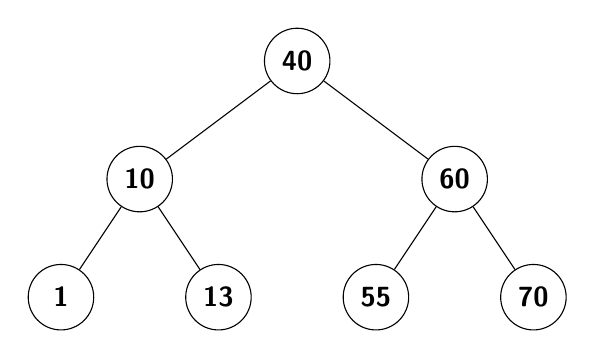
\begin{tikzpicture}[treenode/.style = {align=center, inner sep=1pt, text centered,
        font=\sffamily},
      bst/.style = {treenode, circle, black, font=\sffamily\bfseries, draw=black, text width=2em},level/.style={sibling distance = 4cm/#1,
      level distance = 1.5cm}]
    \node [bst] {40}
        child {node [bst] {10}
            child {node [bst] {1}}
            child {node [bst](n6) {13}}
        }
        child {node [bst] {60}
           child {node[bst] {55}}
            child {node [bst] {70}
            }
        }
    ;
    \end{tikzpicture}
\end{frame}

\begin{frame}[fragile]
    \frametitle{Quiz}
Please draw the resulting tree after deleting 40.


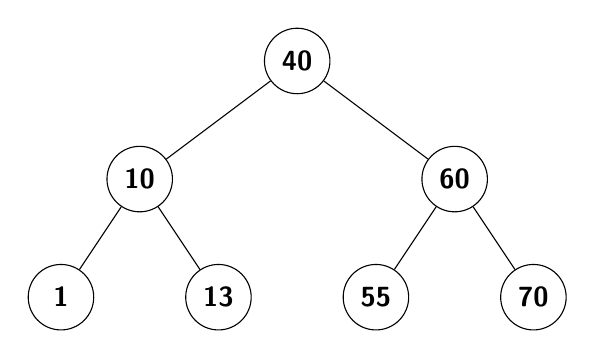
\begin{tikzpicture}[treenode/.style = {align=center, inner sep=1pt, text centered,
    font=\sffamily},
  bst/.style = {treenode, circle, black, font=\sffamily\bfseries, draw=black, text width=2em},level/.style={sibling distance = 4cm/#1,
  level distance = 1.5cm}]
\node [bst] {40}
    child {node [bst] {10}
        child {node [bst] {1}}
        child {node [bst](n6) {13}}
    }
    child {node [bst] {60}
       child {node[bst] {55}}
        child {node [bst] {70}
        }
    }
;
\end{tikzpicture}


\end{frame}

{
    % \usebackgroundtemplate{\transparent{0.3}{\begin{picture}
    %     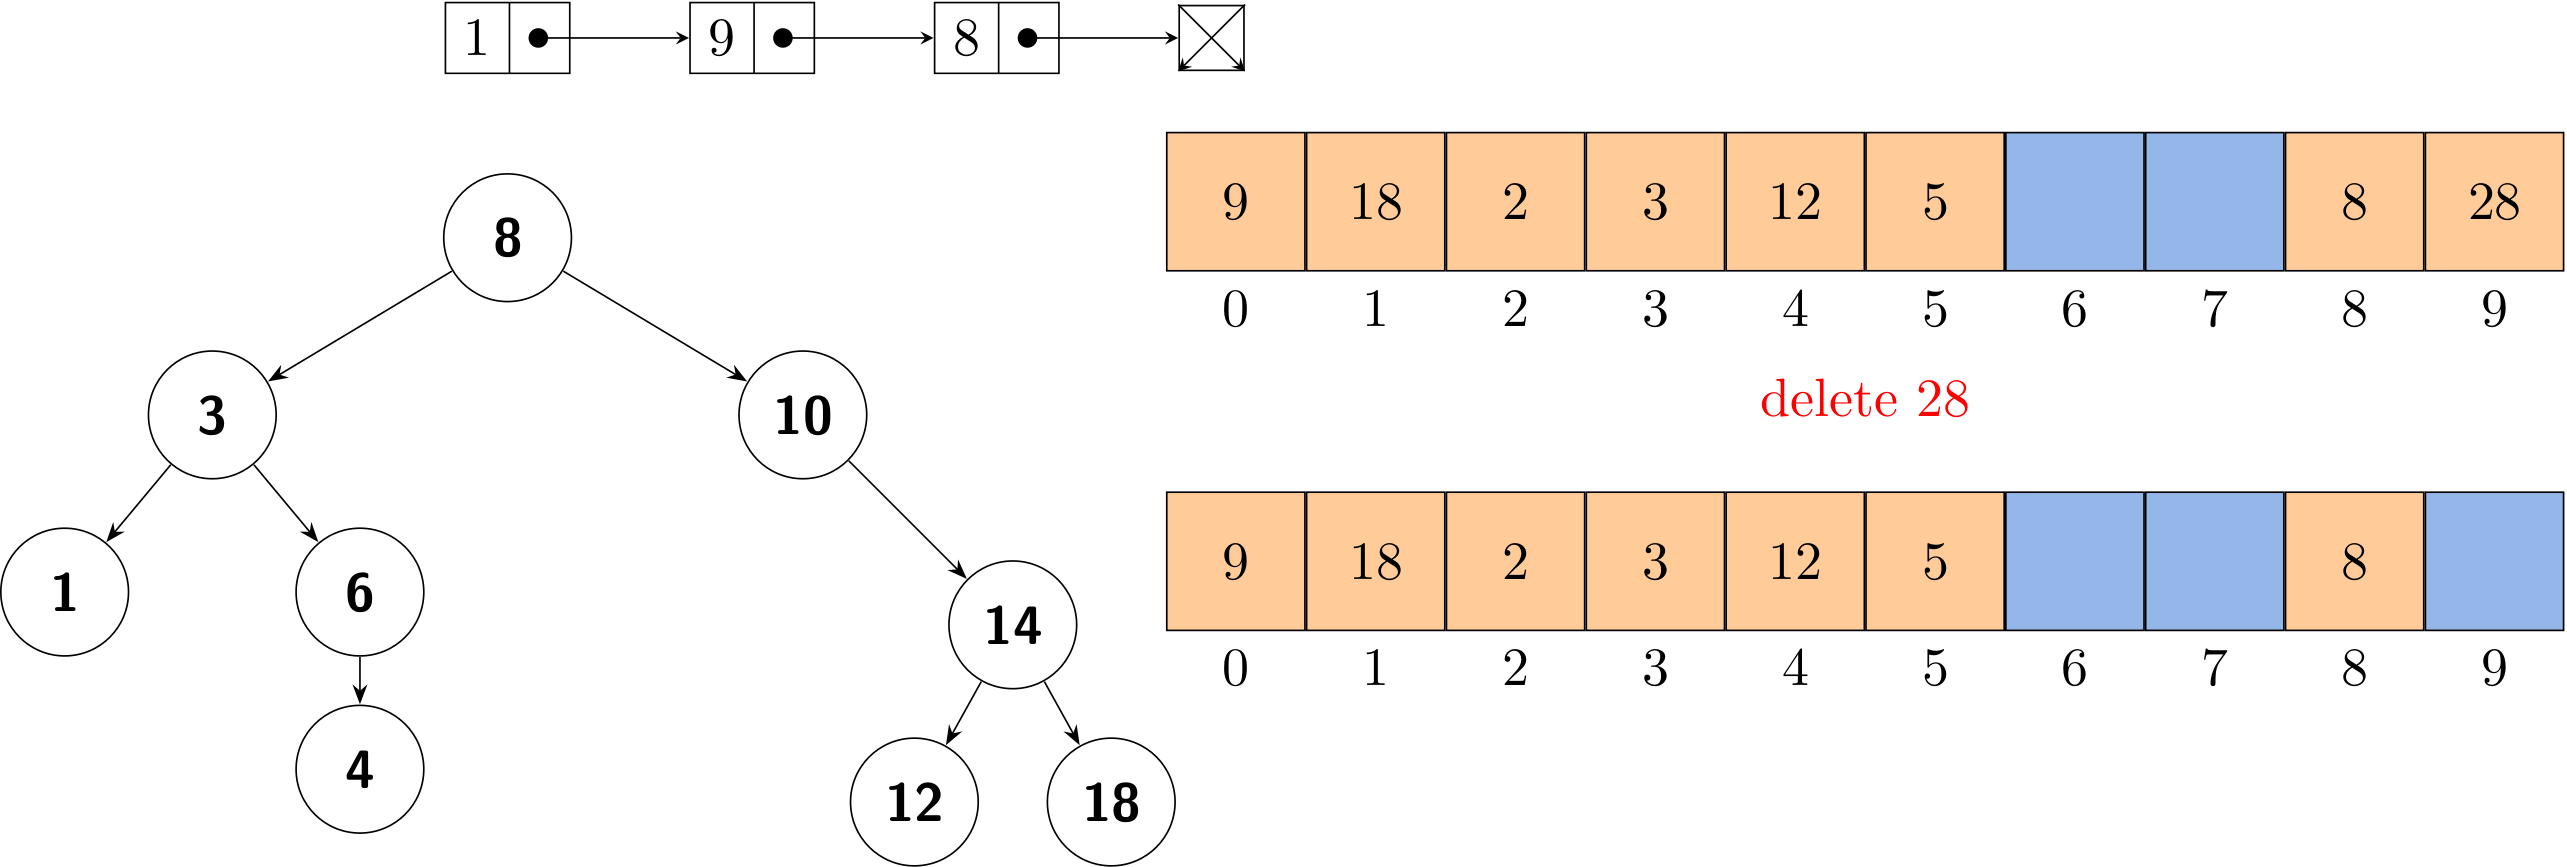
\includegraphics[height=0.7\paperheight]{cover}
    % \end{picture}    
    % }}
\usebackgroundtemplate{
  \tikz[overlay,remember picture] 
  \node[opacity=0.3, at=(current page.south east),anchor=south east, yshift=2cm,xshift=4cm] {
    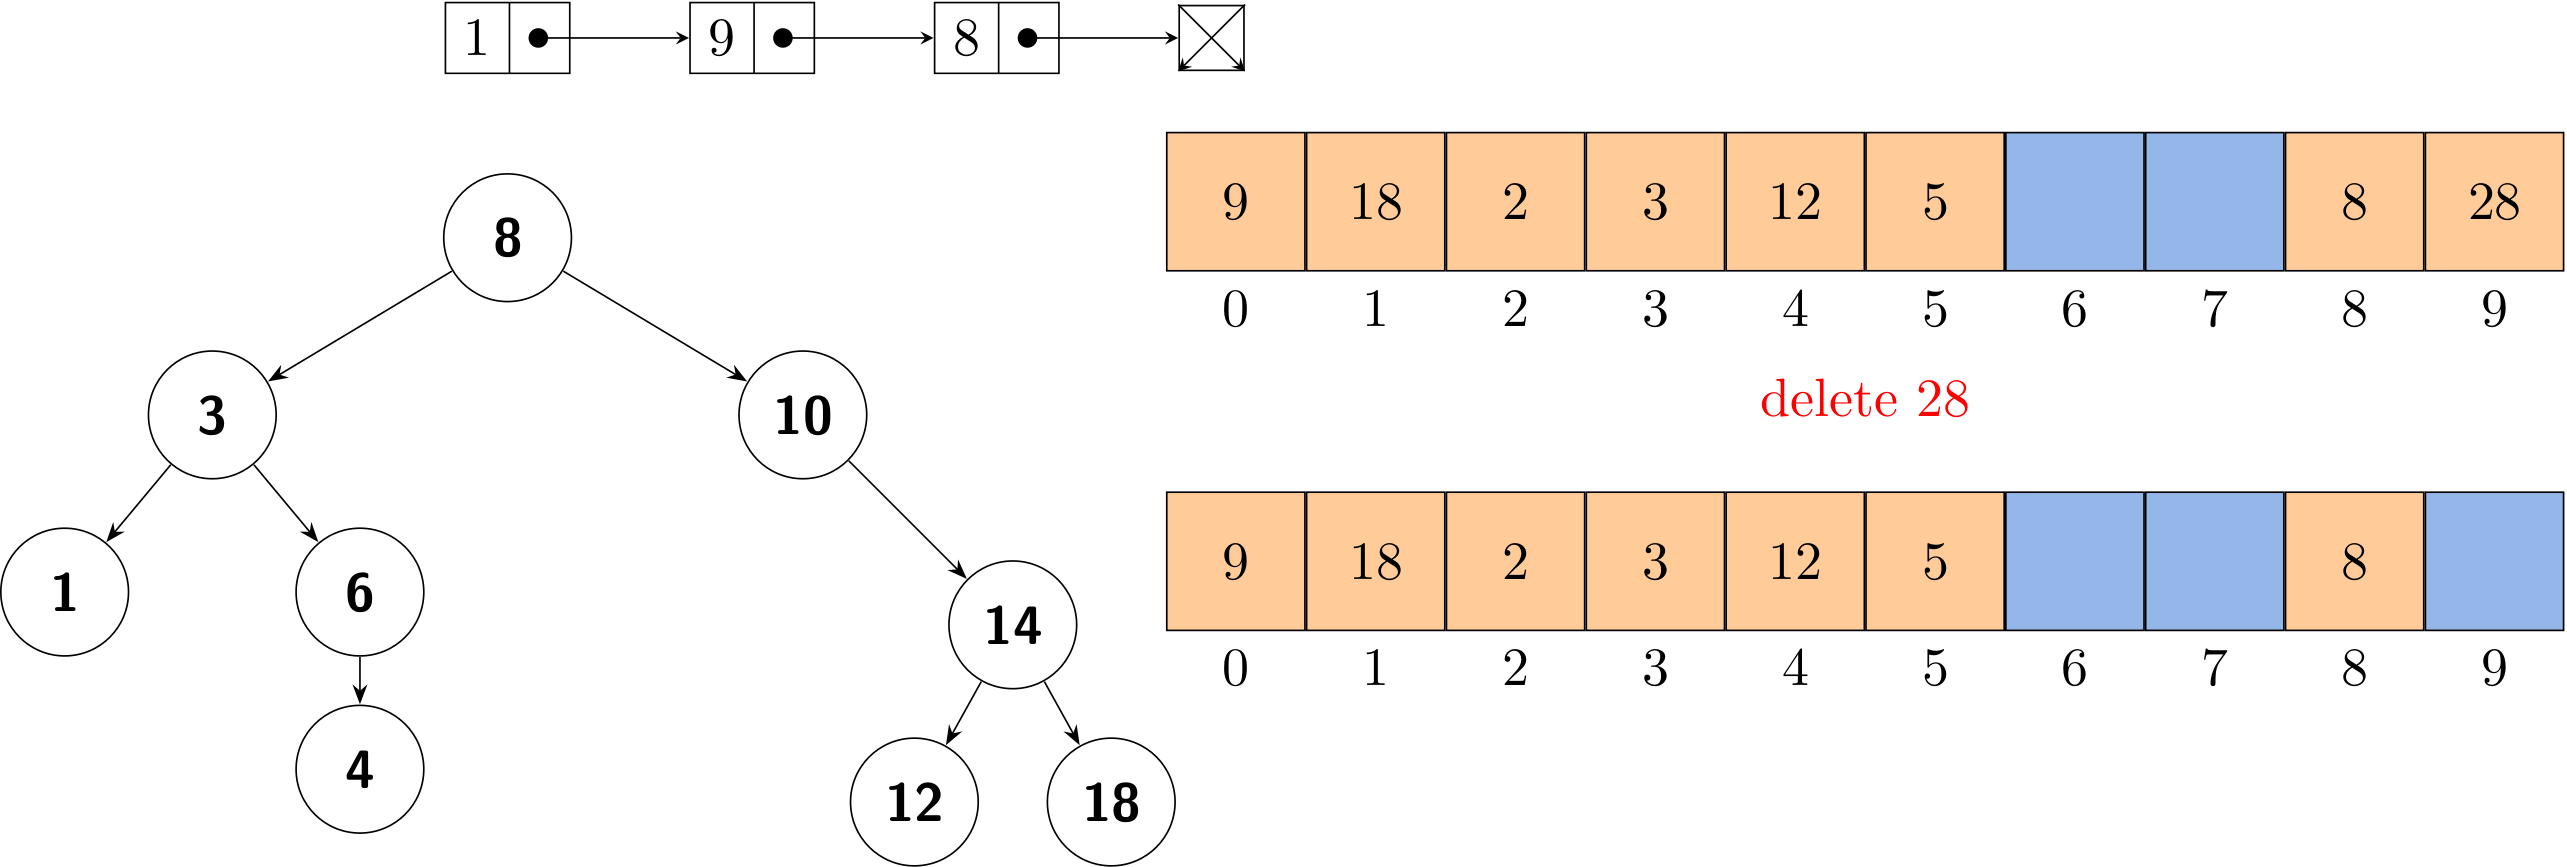
\includegraphics[height=0.6\paperheight]{cover}};
}
    \begin{frame}
        \section{\textcolor{darkmidnightblue}{1. Priority Queue}}
    \end{frame}
}


\begin{frame}
    \frametitle{1.1 Revisit Queue}
A queue is a FIFO data structure. But what if someone is a VIP, can he jump the queue?
    
\begin{center}
    
\includegraphics[height=.4\paperheight]{week4/atm}
\end{center} 
In practice, the item with the highest \alert{priority} will be processed first.
\end{frame}

\begin{frame}
    \frametitle{More Examples}

\begin{itemize}
    \item \faIcon{mobile-alt} A cellphone is capable of running several applications at the same time. In fact, each application is assigned a priority, then OS always chooses to \underline{process the highest-priority event}.
    \item \faIcon{laptop} When your computer is limited in memory or CPU resource, it is likely to \underline{kill or pause the application with the lowest-priority}.
\end{itemize}

\end{frame}

\begin{frame}[fragile]
    \frametitle{1.2 Priority Queue}
As for a \textbf{maximum priority queue}, it mainly supports two operations:

\begin{itemize}
    \item \texttt{delMax()} (remove the maximum)
    \item \texttt{insert()}
\end{itemize}

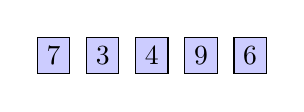
\begin{tikzpicture}
    \matrix [column sep=.2cm, every node/.style={draw, fill=blue!20}] {
        \node {7}; & \node {3}; & \node {4}; & \node {9}; & \node {6}; \\
    };
\end{tikzpicture}

Similarly, we can also design \textbf{minimum priority queues}.
\end{frame}

\begin{frame}
    \frametitle{1.3 Implementation 1: Array-based}
Suppose the array is unordered:

\begin{itemize}
    \item \texttt{insert()}: insert the element at the end.
    \item \texttt{delMax()}: find the largest element, and then remove it.
\end{itemize}

\faIcon{code} Please analyze the time complexity of the two operations. What is the array is ordered?

\end{frame}

\begin{frame}
    
    \begin{table}
        \caption{Time Complexity}
        \begin{tabular}{lrr}
          \toprule
          data structure & insert() & delMax() \\
          \midrule
          ordered array & O(N) & O(1) \\
          unordered array & O(1) & O(N) \\
          \bottomrule
        \end{tabular}
    \end{table}

\faIcon{lightbulb} What if we adopt a linked list as the underlying storage?
\end{frame}

{
\usebackgroundtemplate{
  \tikz[overlay,remember picture] 
  \node[opacity=0.3, at=(current page.north),anchor=north, xshift=4cm] {
    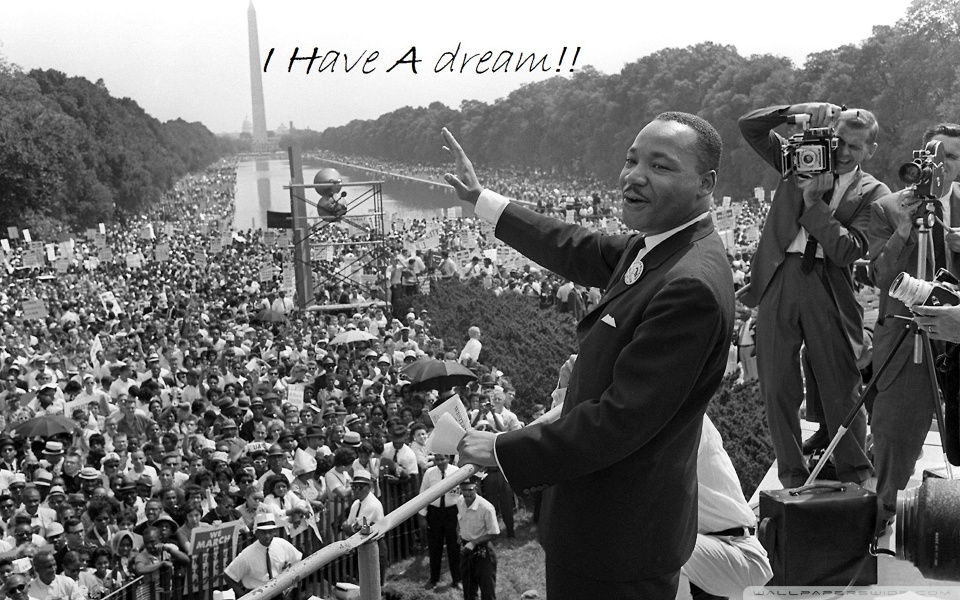
\includegraphics[height=0.6\paperheight]{week10/dream}};
}
\begin{frame}[fragile]
    \frametitle{1.4 I Have A Dream}

that \alert{\textbf{all the operations can be done in constant time}}.    

\pause
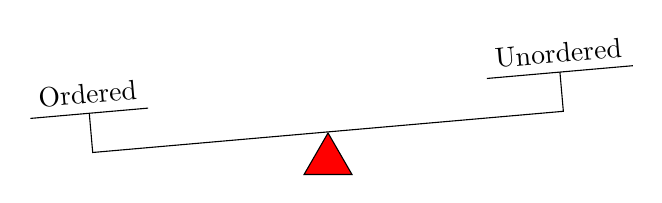
\begin{tikzpicture}[pivot/.style={
    draw, 
    regular polygon, 
    regular polygon sides = 3, 
    fill = red, 
    node distance = 1cm, 
    minimum height = 2em,
    at = {(0,0)}
  }]
    \node [pivot] (a) {};
  
    \begin{scope}[rotate around={5:(a.corner 1)}]
     \draw (a.corner 1) -| ++(-3cm,5mm) node[transform shape,above] (t1) {Ordered};
     \draw (a.corner 1) -| ++(3cm,5mm) node[transform shape,above] (t2) {Unordered};
     \draw (t1.south east) -- (t1.south west);
     \draw (t2.south east) -- (t2.south west);
    \end{scope}
  \end{tikzpicture}

  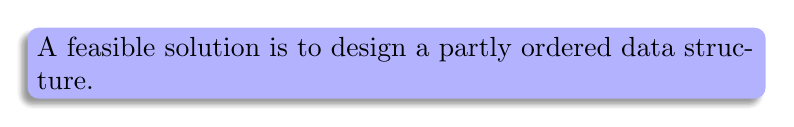
\begin{tikzpicture}
    \node[fill=blue!30,blur shadow={shadow xshift=-0.5ex},
    text width=26em,anchor=south west,rounded corners]
    {A feasible solution is to design a \alert{partly} ordered data structure.};
\end{tikzpicture}

\end{frame}
}

\begin{frame}
    \frametitle{1.5 Heap}

\begin{exampleblock}{Heap-ordered}
    A binary tree is heap-ordered if the key in each node is larger than or equal to the keys in that node's two children (if any).    
\end{exampleblock}

\faIcon{lightbulb} Where is the largest item?


\end{frame}

\begin{frame}[fragile]
    
    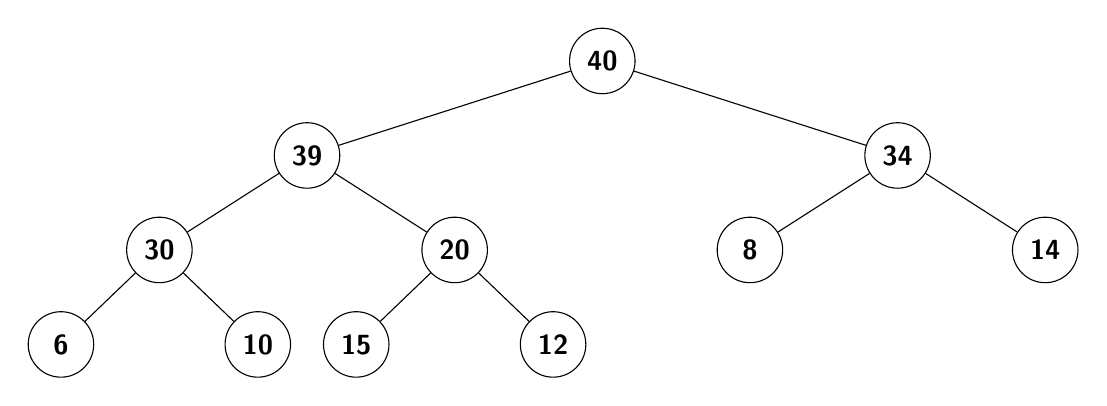
\begin{tikzpicture}[
        treenode/.style = {align=center, inner sep=1pt, text centered,
        font=\sffamily},
      bst/.style = {treenode, circle, black, font=\sffamily\bfseries, draw=black, text width=2em},
        level/.style={sibling distance = 7.5cm/#1,
        level distance = 1.2cm}]
      \node [bst] {40}
          child {node [bst] {39}
              child {node [bst] {30}
                  child {node [bst] {6}}
                  child {node [bst] {10}}
              }
              child {node [bst] {20}
                  child {node [bst] {15}}
                  child {node [bst] {12}}
              }
          }
          child { node [bst] {34}
              child{node [bst] {8}}
              child{node [bst] {14}}
          }
      ;
      \end{tikzpicture}

\faIcon{code} Can you take a guess about the time complexities of a priority queue which is implemented by a heap-ordered binary tree?
\end{frame}

\begin{frame}

    \section{\textcolor{darkmidnightblue}{2. Heap}} 
\end{frame}


\begin{frame}[fragile]
    \frametitle{Task}
\faIcon{search} Please try to understand the definition of a \alert{complete tree} by searching from the Internet.
    
Which of the following are \underline{complete trees}?

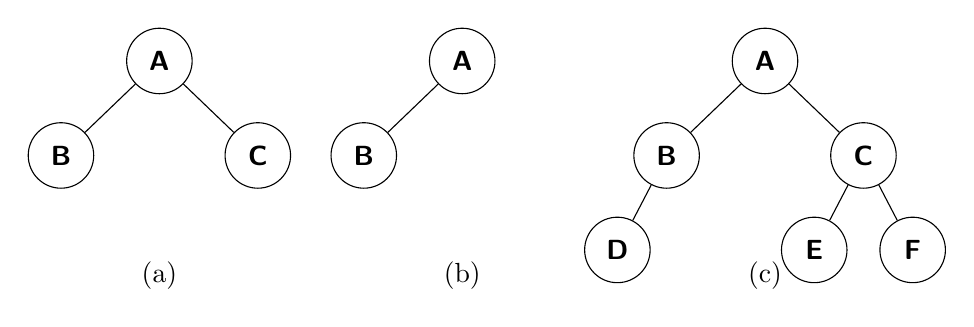
\begin{tikzpicture}[
    treenode/.style = {align=center, inner sep=1pt, text centered,
    font=\sffamily},
  bst/.style = {treenode, circle, black, font=\sffamily\bfseries, draw=black, text width=2em},
    level/.style={sibling distance = 2.5cm/#1,
    level distance = 1.2cm}, noline/.style={edge from parent/.style={black, line width=0.2mm}}]
  \node [bst] (root1) {A}
      child {node [bst] {B}}
      child {node [bst] {C}}
  ;
  \node [below=of root1, yshift=-1cm] {(a)};

  \node [bst, right=of root1, xshift=2cm] (root2) {A}
    child {node [bst] {B}}
    child [noline] {node {}}
  ;
  \node [below=of root2, yshift=-1cm] {(b)};

  \node [bst, right=of root2, xshift=2cm] (root3) {A}
    child {node [bst] {B}
        child {node [bst] {D}}
        child [noline] {node {}}
    }
    child {node [bst] {C}
        child {node [bst] {E}}
        child {node [bst] {F}}
    }
  ;
  \node [below=of root3, yshift=-1cm] {(c)};
  \end{tikzpicture}

\end{frame}

\begin{frame}[fragile]
    \frametitle{2.1 Compact Array}
    We represent \alert{complete binary trees} sequentially within an array by putting the nodes in \textbf{level order}, with the root at position 1, its children at positions 2 and 3, their children in positions 4, 5, 6 and 7, and so on.

\begin{columns}
    \column{.4\textwidth}
    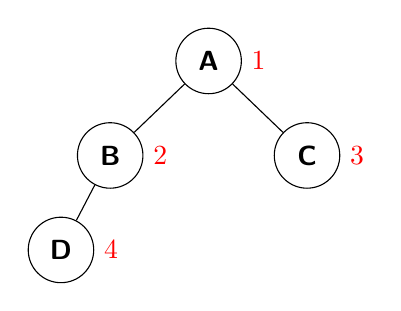
\begin{tikzpicture}[
        treenode/.style = {align=center, inner sep=1pt, text centered,
        font=\sffamily},
      bst/.style = {treenode, circle, black, font=\sffamily\bfseries, draw=black, text width=2em},
        level/.style={sibling distance = 2.5cm/#1,
        level distance = 1.2cm}, noline/.style={edge from parent/.style={black, line width=0.2mm}}]
      \node [bst] (a) {A}
          child {node [bst] (b) {B}
            child {node [bst] (d) {D}}
            child [noline] {node {}}
          }
          child {node [bst] (c) {C}}
      ;
      \node[right=of a, red, xshift=-1cm] {1};
      \node[right=of b, red, xshift=-1cm] {2};
      \node[right=of c, red, xshift=-1cm] {3};
      \node[right=of d, red, xshift=-1cm] {4};
    \end{tikzpicture}
    \column{.6\textwidth}
    \begin{table}
        \begin{tabular}{llllll}
          \toprule
          i & 0 & 1 & 2 & 3 & 4 \\
          \midrule
          a[i] & & A & B & C & D \\
          \bottomrule
        \end{tabular}
    \end{table}
    \faIcon{lightbulb} What is the advantage of using arrays to represent a complete binary tree?
\end{columns}

\end{frame}

\begin{frame}[fragile]
    \begin{columns}
        \column{.4\textwidth}
        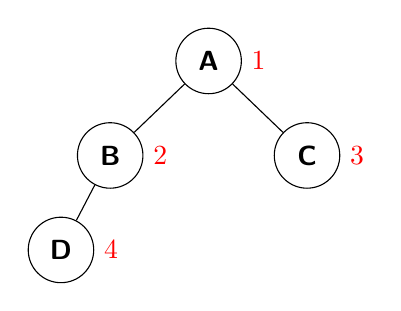
\begin{tikzpicture}[
            treenode/.style = {align=center, inner sep=1pt, text centered,
            font=\sffamily},
          bst/.style = {treenode, circle, black, font=\sffamily\bfseries, draw=black, text width=2em},
            level/.style={sibling distance = 2.5cm/#1,
            level distance = 1.2cm}, noline/.style={edge from parent/.style={black, line width=0.2mm}}]
          \node [bst] (a) {A}
              child {node [bst] (b) {B}
                child {node [bst] (d) {D}}
                child [noline] {node {}}
              }
              child {node [bst] (c) {C}}
          ;
          \node[right=of a, red, xshift=-1cm] {1};
          \node[right=of b, red, xshift=-1cm] {2};
          \node[right=of c, red, xshift=-1cm] {3};
          \node[right=of d, red, xshift=-1cm] {4};
        \end{tikzpicture}
        \column{.6\textwidth}
        \begin{table}
            \begin{tabular}{llllll}
              \toprule
              i & 0 & 1 & 2 & 3 & 4 \\
              \midrule
              a[i] & & A & B & C & D \\
              \bottomrule
            \end{tabular}
        \end{table}
    \end{columns}
Important findings:

\begin{itemize}
    \item The parent of the node in position $k$ is position $\lfloor k/2 \rfloor$.
    \item The two children of the node in position $k$ are in positions $2k$ and $2k + 1$.
\end{itemize}
\end{frame}

\begin{frame}
    \frametitle{2.2 Binary Heap}
\begin{exampleblock}{Binary Heap}
A binary heap is a complete binary tree that satisfies the heap property.    
\end{exampleblock}
For brevity, we will use \alert{heap} when referring to a binary heap.

\faIcon{code} Please prove the height of a complete binary tree of size $N$ is $\lfloor \log{N} \rfloor$.

\end{frame}

\begin{frame}[fragile]
    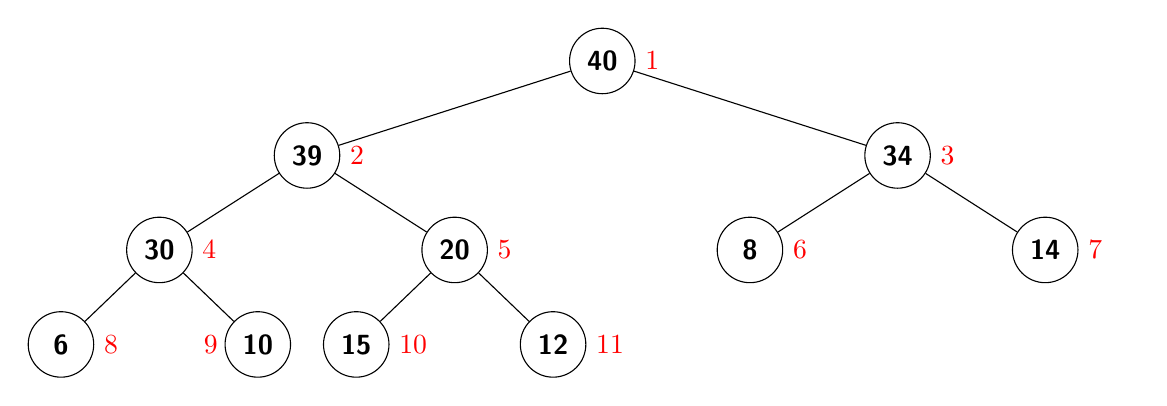
\begin{tikzpicture}[
        treenode/.style = {align=center, inner sep=1pt, text centered,
        font=\sffamily},
      bst/.style = {treenode, circle, black, font=\sffamily\bfseries, draw=black, text width=2em},
        level/.style={sibling distance = 7.5cm/#1,
        level distance = 1.2cm}, txt/.style = {text width=1.5em, red}]
        \node (n40) [bst] {40}
        child {node (n39) [bst] {39}
            child {node (n30) [bst] {30}
                child {node (n6) [bst] {6}}
                child {node (n10) [bst] {10}}
            }
            child {node (n20) [bst] {20}
                child {node (n15) [bst] {15}}
                child {node (n12) [bst] {12}}
            }
        }
        child { node (n34) [bst] {34}
            child{node (n8) [bst] {8}}
            child{node (n14) [bst] {14}}
        }
    ;
    \node [right, txt] at (n40.east) {1};
    \node [right, txt] at (n39.east) {2};
    \node [right, txt] at (n34.east) {3};
    \node [right, txt] at (n30.east) {4};
    \node [right, txt] at (n20.east) {5};
    \node [right, txt] at (n8.east) {6};
    \node [right, txt] at (n14.east) {7};
    \node [right, txt] at (n6.east) {8};
    \node [txt] at (n10.west) {9};
    \node [right, txt] at (n15.east) {10};
    \node [right, txt] at (n12.east) {11};
      \end{tikzpicture}

If the priority queue is implemented by a heap, its time complexity can be summarized:

    \begin{table}
        \begin{tabular}{lll}
          \toprule
          data structure & insert() & delMax() \\
          \midrule
          heap & $O(\log{N})$ & $O(\log{N})$ \\
          \bottomrule
        \end{tabular}
    \end{table}

\end{frame}

\begin{frame}[fragile]
    \frametitle{2.3 insert()}

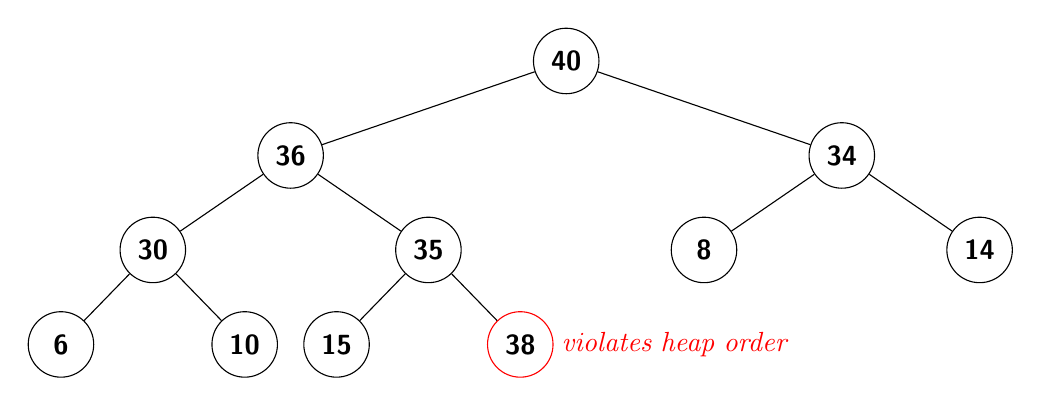
\begin{tikzpicture}[  treenode/.style = {align=center, inner sep=1pt, text centered,
    font=\sffamily},
  bst/.style = {treenode, circle, black, font=\sffamily\bfseries, draw=black, text width=2em}, 
  sst/.style = {treenode, circle, black, font=\sffamily\bfseries, draw=red, text width=2em}, 
  txt/.style = {text width=1.5em, red},
  redline/.style={edge from parent/.style={red,very thick,latex-, draw}},
  rugularline/.style={edge from parent/.style={black, line width=0.2mm, draw}},
  noline/.style={edge from parent/.style={black, line width=0.2mm}},
  level/.style={sibling distance = 7cm/#1,
  level distance = 1.2cm}
  ]
  \node [bst] (2n1) {40}
  child {node [bst] {36}
      child {node [bst] {30}
          child {node [bst] {6}}
          child {node [bst] {10}}
      }
      child {node [bst] {35}
          child {node [bst] {15}}
          child {node (2key38) [sst] {38}}
      }
  }
  child { node [bst] {34}
      child{node [bst] {8}}
      child{node [bst] {14}}
  }
;
\node [right, txt, text width=4cm, xshift=4mm] at (2key38) {\textit{violates heap order}};
\end{tikzpicture}

\end{frame}

\begin{frame}[fragile]
It can be fixed by \alert{swim} (bottom-up reheapify), which is performed by \textbf{swapping with its parent}.
    
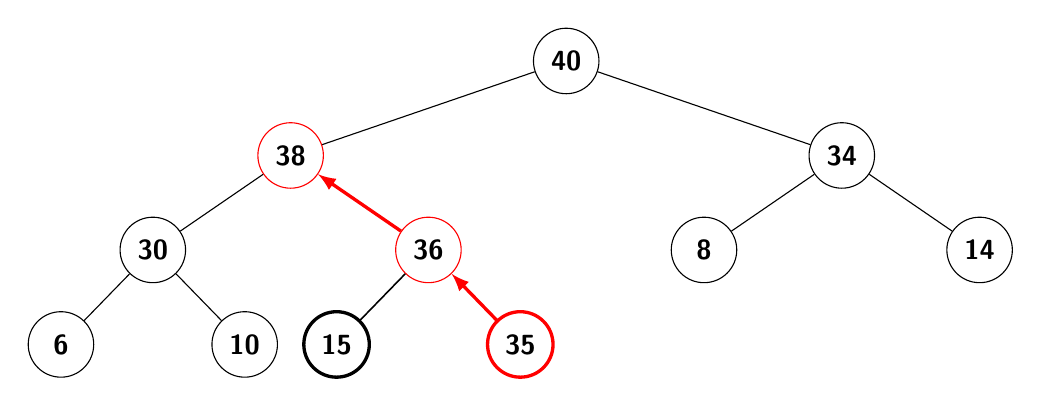
\begin{tikzpicture}[  treenode/.style = {align=center, inner sep=1pt, text centered,
    font=\sffamily},
  bst/.style = {treenode, circle, black, font=\sffamily\bfseries, draw=black, text width=2em}, 
  sst/.style = {treenode, circle, black, font=\sffamily\bfseries, draw=red, text width=2em}, 
  txt/.style = {text width=1.5em, red},
  redline/.style={edge from parent/.style={red,very thick,latex-, draw}},
  rugularline/.style={edge from parent/.style={black, line width=0.2mm, draw}},
  noline/.style={edge from parent/.style={black, line width=0.2mm}},
  level/.style={sibling distance = 7cm/#1,
  level distance = 1.2cm}
  ]
  \node [bst] (3n1) {40}
  child {node [sst] {38}
      child {node [bst] {30}
          child {node [bst] {6}}
          child {node [bst] {10}}
      }
      child [redline] {node [sst] {36}
          child [rugularline] {node [bst] {15}}
          child [redline] {node  [sst] {35}}
      }
  }
  child { node [bst] {34}
      child{node [bst] {8}}
      child{node [bst] {14}}
  }
;
\end{tikzpicture}

\end{frame}

\begin{frame}[fragile]
\scalebox{.9}{
    \begin{algorithm}[H]
        \caption{swim(k)}
        \KwIn{The position $k$ in $qp$}
        \While{k $>$ 1 and \textnormal{less(}k/2, k\textnormal{)}}{
            swap($k/2$, $k$) \\
            $k\gets k/2$
        }
        \end{algorithm}
}

\begin{minted}[bgcolor=LightGray,]{java}
// N is the size of pq
public void insert(Key v) {
    pq[++N] = v;
    swim(N);
}
\end{minted}

\end{frame}

\begin{frame}[fragile]
    \frametitle{2.4 delMax()}
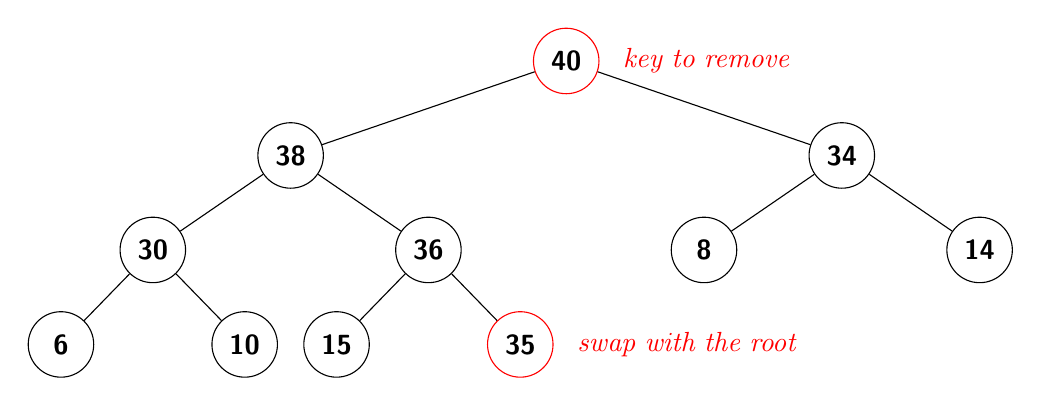
\begin{tikzpicture}[  treenode/.style = {align=center, inner sep=1pt, text centered,
    font=\sffamily},
  bst/.style = {treenode, circle, black, font=\sffamily\bfseries, draw=black, text width=2em}, 
  sst/.style = {treenode, circle, black, font=\sffamily\bfseries, draw=red, text width=2em}, 
  txt/.style = {text width=1.5em, red},
  redline/.style={edge from parent/.style={red,very thick,-latex, draw}},
  rugularline/.style={edge from parent/.style={black, line width=0.2mm, draw}},
  noline/.style={edge from parent/.style={black, line width=0.2mm}},
  level/.style={sibling distance = 7cm/#1,
  level distance = 1.2cm}
  ]
  \node [sst] (n1) {40}
  child {node [bst] {38}
      child {node [bst] {30}
          child {node [bst] {6}}
          child {node [bst] {10}}
      }
      child  {node [bst] {36}
          child {node [bst] {15}}
          child {node (key35) [sst] {35}}
      }
  }
  child { node [bst] {34}
      child{node [bst] {8}}
      child{node [bst] {14}}
  }
;

\node [right, txt, text width=4cm, xshift=6mm] at (n1) {\textit{key to remove}};
\node [right, txt, text width=4cm, xshift=6mm] at (key35) {\textit{swap with the root}};
\end{tikzpicture}
\end{frame}

\begin{frame}[fragile]
It can be fixed by \alert{sink} (top-down reheapify) by \textbf{swapping with its child}.

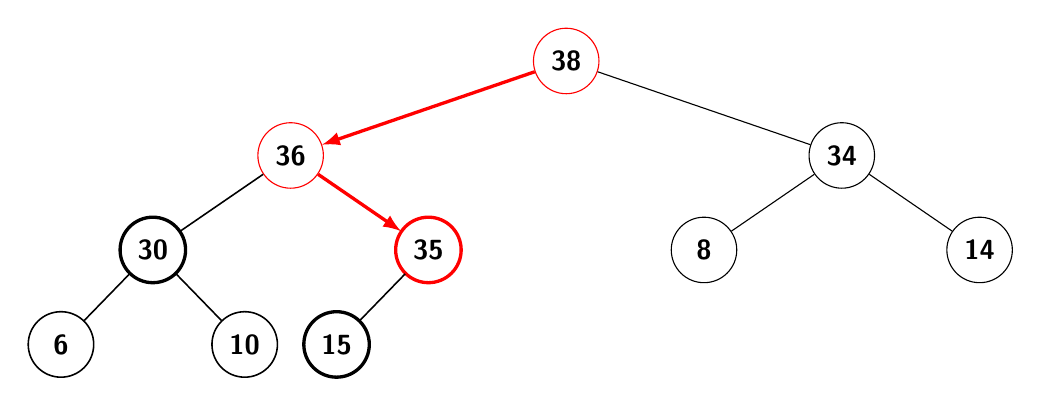
\begin{tikzpicture}[treenode/.style = {align=center, inner sep=1pt, text centered,
    font=\sffamily},
  bst/.style = {treenode, circle, black, font=\sffamily\bfseries, draw=black, text width=2em}, 
  sst/.style = {treenode, circle, black, font=\sffamily\bfseries, draw=red, text width=2em}, 
  txt/.style = {text width=1.5em, red},
  redline/.style={edge from parent/.style={red,very thick,-latex, draw}},
  rugularline/.style={edge from parent/.style={black, line width=0.2mm, draw}},
  noline/.style={edge from parent/.style={black, line width=0.2mm}},
  level/.style={sibling distance = 7cm/#1,
  level distance = 1.2cm}
  ]
  \node [sst] (3n1) {38}
  child [redline] {node [sst] {36}
      child [rugularline] {node [bst] {30}
          child {node [bst] {6}}
          child {node [bst] {10}}
      }
      child  {node [sst] {35}
          child [rugularline] {node [bst] {15}}
          child [noline] {node {}}
      }
  }
  child { node [bst] {34}
      child{node [bst] {8}}
      child{node [bst] {14}}
  }
;

\end{tikzpicture}

\faIcon{lightbulb} Given a node $x$ and its children $x.left$, $x.right$ violating the heap property, how to perform the \textbf{swapping}?
\end{frame}

\begin{frame}[fragile]
    \scalebox{.8}{
        \begin{algorithm}[H]
            \caption{sink(k)}
            \KwIn{The position $k$ in $qp$}
            \While{2 * k $\leq$ N}{
                $j\gets 2*k$ \tcp{left child}
                \If{j $<$ N and \textnormal{less(}j, j+1\textnormal{)}}{
                    $j\gets j + 1$
                }
                \tcp{$j$ is the larger child} 
                \If{not \textnormal{less(}k, j\textnormal{)}}{break}
                swap($k$, $j$) \\
                $k\gets j$
            }
        \end{algorithm}        
    }

\end{frame}

\begin{frame}[fragile]
    Try to fill in the blanks.
    \begin{minted}[bgcolor=LightGray,]{java}
public Key delMax() {
    Key max = pq[1];
    _______________
    pq[N+1] = null;
    _______________
    return max;
}
    \end{minted}
\end{frame}

\begin{frame}[fragile]
    \frametitle{2.5 Heap Sort}
We can use the priority queue to develop a sorting algorithm.

\begin{minted}[bgcolor=LightGray, baselinestretch=1]{java}
public static void sort(Comparable[] a){
     int N = a.length;
     for (int k = N/2; k >= 1; k--)
        sink(a, k, N);
     while (N > 1) {
        swap(a, 1, N--);
        sink(a, 1, N);
     }
}
\end{minted} 
\end{frame}

\begin{frame}[fragile]
    \frametitle{2.6 Built-in Priority Queues}
Again, you don't have to design a priority queue from the scratch.

\begin{itemize}
    \item \faIcon{java} \href{https://docs.oracle.com/en/java/javase/11/docs/api/java.base/java/util/PriorityQueue.html}{java.util.PriorityQueue}: it is a minimum priority queue.
    \item \faIcon{python} \href{https://docs.python.org/3/library/heapq.html}{heapq}: it is also a minimum priority queue.
\end{itemize}

\begin{minted}[bgcolor=LightGray, baselinestretch=.9]{python}
pq = []
heapq.heappush(pq, 1)
heapq.heappush(pq, 4)
heapq.heappush(pq, 0)
heapq.heappush(pq, 6)
heapq.heappush(pq, 3)
print(heapq.heappop(pq))  # 0
print(pq[0])  # 1
\end{minted} 

\end{frame}

\begin{frame}[fragile]
\faIcon{lightbulb} How to use \texttt{heapq} or \texttt{java.util.PriorityQueue} as a \textbf{max heap}? For simplicity, assume that keys are integers.
    
\pause

\begin{minted}[bgcolor=LightGray, baselinestretch=1.1]{python}
class MaxPQ:
    def __init__(self):
        self._pq = []
    
    def insert(self, e):
        heapq.heapush(self._pq, -e)
    
    def delMax(self):
        return -heapq.heappop(self._pq)
\end{minted}

\end{frame}

\begin{frame}

    \section{\textcolor{darkmidnightblue}{Conclusion}}
    \begin{itemize}
        \item Priority Queue
        \item Heap and Heap Sort
    \end{itemize}
\end{frame}


\begin{frame}
    \frametitle{Homework 6}
\begin{enumerate}
    \item Ask a question about data structures. (10 marks)
    \item Ex 13, Chapter 4 (Bonus). (10 marks) 
\end{enumerate}
\end{frame}

\end{document}